\documentclass[tikz,border=7pt]{standalone}
\usetikzlibrary{matrix,fit,positioning, arrows.meta,
  decorations.pathreplacing, backgrounds} 
\begin{document}
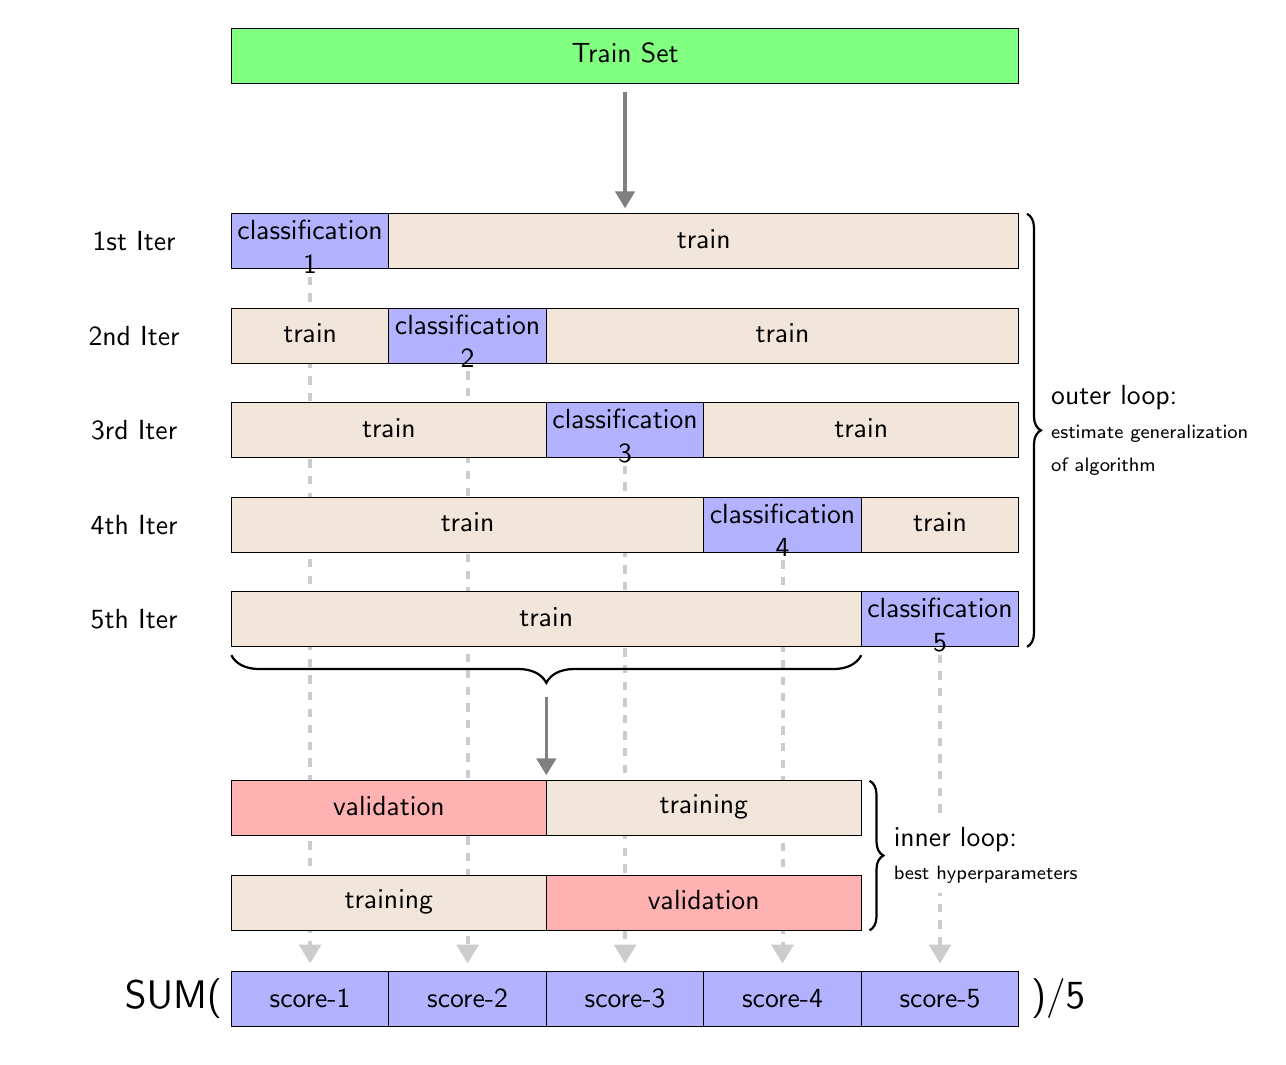
\begin{tikzpicture}[font=\sffamily,
%   Fold/.style={/utils/exec=\stepcounter{Fold}
% \pgfmathtruncatemacro{\itest}{ifthenelse(mod(\number\value{Fold},5)==int(1+\number\value{Fold}/5)
% || \number\value{Fold}==25,1,0)}
% \pgfmathsetmacro{\mycol}{{\LstCol}[\itest]},fill=\mycol,draw,
% node contents={Fold \pgfmathparse{int(mod(\number\value{Fold}-1,5)+1)}\pgfmathresult}
% },
  standard/.style={inner sep=0pt,align=center,draw,%text
    % height=1.25em,
    minimum height = 7mm,
    text depth=0.5em},
  decoration={brace, amplitude=5pt},
  oneblock/.style={transform shape,minimum width=1cm,draw}]
    \matrix (M) [
        matrix of nodes,
        nodes={
%          text height=1.25em,
%          text depth=2cm,
            minimum height = 7mm,
            minimum width = 2cm,
           outer sep=0,
           anchor=center,
           fill=brown!20 % <-added
        },
        column 1/.style={
            nodes={draw=none,fill=none}, % <-- added fill=none
            minimum width = 4cm
          },
        column 7/.style={
            nodes={draw=none,fill=none,align=left}, % <-- added fill=none
            minimum width = 4cm
        },
        row sep=5mm, column sep = 0,%column sep=-\pgflinewidth,
        nodes in empty cells,
        e/.style={draw=none,fill=blue!30},
        e_in/.style={draw=none,fill=red!30},
        t_in/.style={draw=none,fill=brown!20},        
        alignleft/.style={draw=none, fill=none,align=left}
      ]
      {
        1st Iter & |[e]| & & & & &|[draw=none, fill=none]|\\
        2nd Iter & & |[e]| & & & &|[draw=none, fill=none]| \\
        3rd Iter & & & |[e]| & & &|[draw=none, fill=none]| \\
        4th Iter & & & & |[e]| & &|[draw=none, fill=none]| \\        
        5th Iter & & & & & |[e]| &|[draw=none, fill=none]|\\
        |[draw=none,fill=none]| &|[draw=none, fill=none]|
        &|[draw=none, fill=none]| & |[draw=none,
        fill=none]|&|[draw=none, fill=none]| &|[draw=none, fill=none]|
        &|[draw=none, fill=none]|\\
        & |[e_in]|&|[e_in]|& & & |[draw=none, fill=none]|&|[draw=none,
        fill=none]|\\
        & & & |[e_in]|&|[e_in]|& |[draw=none, fill=none]|&|[draw=none,
        fill=none]|\\
        {\hspace*{1cm}\Large SUM(} & |[e]|score-1& |[e]|score-2& |[e]|score-3&
        |[e]|score-4&|[e]|score-5 & {\Large )/5\hspace*{1cm}}\\
      };
      \node[fit=(M-1-3) (M-1-6), standard,fill=none, draw]{train};
      \node[fit=(M-1-2) (M-1-2), standard, fill=none, draw]{classification 1};
      \node[fit=(M-2-2) (M-2-2), standard, fill=none, draw]{train};
      \node[fit=(M-2-3) (M-2-3), standard, fill=none, draw]{classification 2};
      \node[fit=(M-2-4) (M-2-6), standard, fill=none, draw]{train};
      \node[fit=(M-3-2) (M-3-3), standard, fill=none, draw]{train};
      \node[fit=(M-3-4) (M-3-4), standard, fill=none, draw]{classification 3};
      \node[fit=(M-3-5) (M-3-6), standard, fill=none, draw]{train};
      \node[fit=(M-4-2) (M-4-4), standard, fill=none, draw]{train};
      \node[fit=(M-4-5) (M-4-5), standard, fill=none, draw]{classification 4};
      \node[fit=(M-4-6) (M-4-6), standard, fill=none, draw]{train};
      \node[fit=(M-5-2) (M-5-5), standard, fill=none, draw]{train};
      \node[fit=(M-5-6) (M-5-6), standard, fill=none, draw]{classification 5};
      \node[fit=(M-7-2) (M-7-3), standard, fill=none,
      draw]{validation};
      \node[fit=(M-7-4) (M-7-5), standard, fill=none, draw]{training};
      \node[fit=(M-8-2) (M-8-3), standard, fill=none,
      draw]{training};
      \node[fit=(M-8-4) (M-8-5), standard, fill=none,
      draw]{validation};
      % lines for SUM(scores):
      \node[fit=(M-9-2) (M-9-2), standard, fill=none, draw]{};
      \node[fit=(M-9-3) (M-9-3), standard, fill=none, draw]{};
      \node[fit=(M-9-4) (M-9-4), standard, fill=none, draw]{};
      \node[fit=(M-9-5) (M-9-5), standard, fill=none, draw]{};
      \node[fit=(M-9-6) (M-9-6), standard, fill=none, draw]{};                  
      % \draw (M-1-3.north west) ++(0,2mm) coordinate (LT) edge[|<->|, >= latex] node[above]{Train} (LT-|M-1-6.north east); % changed 5 to 7
      %  \draw (M-1-2.north west) ++(0,2mm) coordinate (LT) edge[|<->|,
      %  >= latex] node[above]{Test} (LT-|M-1-2.north east);
       % geschweifte Klammer auf rechter Seite
       \draw[thick, decorate] ([yshift=0pt, xshift=3pt]M-1-6.north east) -- ([yshift=-0pt, xshift=3pt]M-5-6.south east)
       node[midway,right, xshift=5pt,align=left]{outer
         loop:\\\scriptsize estimate
       generalization\\\scriptsize of algorithm};
       \draw[thick,decorate, decoration={brace,amplitude=10pt,mirror}] ([yshift=-3pt, xshift=0pt]M-5-2.south
       west) -- ([yshift=-3pt, xshift=0pt]M-5-5.south east)
       node[midway](brace2){};
       % arrow
       \draw[->][black!50, line
           width=1.2pt,-Triangle](brace2.south) ++(0,-4mm)--
           ([yshift=2pt]M-7-4.north west);
       \draw[thick,decorate, decoration={brace, amplitude=5pt}]
           ([yshift=0pt, xshift=3pt]M-7-5.north east) -- ([yshift=0pt,
           xshift=3pt]M-8-5.south east)node[midway,right, xshift=5pt, align=left,fill=white]
           {inner loop:\\ \scriptsize best hyperparameters};
       % big bars above matrix
       \node[fit=(M-1-2) (M-1-6), fill=green!50,
       yshift=2cm, standard, anchor=south](trs) {Train Set};
       \draw[->][black!50, line
           width=1.2pt,-Triangle](trs.south) ++(0,-1mm)--
           ([yshift=2pt]M-1-4.north);
       %\node[oneblock, minimum height = 7mm, minimum width = 2cm,
       % anchor=west,right=of M-2-6,fill=brown!20,outer sep=0mm] (A1)
       % {Train};
       % \node[oneblock, minimum height = 7mm, minimum width = 2cm,
       % anchor=east,right=of M-3-6,fill=blue!30,outer sep=0mm] (A2) {Test};       
      % dots
      %\node [below=3pt] at (M-3-5.south east) {$\cdots$};

      % fold labels and arrows
       \foreach [
             count=\row,
             evaluate={\col=ifthenelse(\row==99, % if fourth row
                                       int(\row+3), % use seventh column
                                       int(\row+1)) % else use column row+1
                       }
                ] \txt in {1,2,3,4,5}
         {
           % \node [below] at (M-\row-\col.south) {Fold-\txt};
           %\draw[->][black!50, line
           %width=0.5mm,-Triangle](M-\row-\col.south) -- (M-7-\col.north);
           % \draw [black!30,line width=1mm,-Triangle] (M-\row-6.east) ++(2mm,0) -- ++(7mm,0) node[black, right] {$E_{\txt}$}; 
         }
         \begin{scope}[on background layer]
           \draw[->][black!20, line
           width=0.5mm,-Triangle,dashed](M-1-2.south) ++(0,-1mm)--([yshift=1mm]M-9-2.north);
           \draw[->][black!20, line
           width=0.5mm,-Triangle,dashed](M-2-3.south) ++(0,-1mm)--([yshift=1mm]M-9-3.north);
           \draw[->][black!20, line
           width=0.5mm,-Triangle,dashed](M-3-4.south) ++(0,-1mm)--([yshift=1mm]M-9-4.north);
           \draw[->][black!20, line
           width=0.5mm,-Triangle,dashed](M-4-5.south) ++(0,-1mm)--([yshift=1mm]M-9-5.north);
           \draw[->][black!20, line
           width=0.5mm,-Triangle,dashed](M-5-6.south) ++(0,-1mm)--([yshift=1mm]M-9-6.north);
         \end{scope}
         
  \end{tikzpicture}
\end{document}
%%% Local Variables:
%%% mode: latex
%%% TeX-master: t
%%% End:
